\documentclass[12pt,]{article}
\usepackage{lmodern}
\usepackage{amssymb,amsmath}
\usepackage{ifxetex,ifluatex}
\usepackage{fixltx2e} % provides \textsubscript
\ifnum 0\ifxetex 1\fi\ifluatex 1\fi=0 % if pdftex
  \usepackage[T1]{fontenc}
  \usepackage[utf8]{inputenc}
\else % if luatex or xelatex
  \ifxetex
    \usepackage{mathspec}
  \else
    \usepackage{fontspec}
  \fi
  \defaultfontfeatures{Ligatures=TeX,Scale=MatchLowercase}
\fi
% use upquote if available, for straight quotes in verbatim environments
\IfFileExists{upquote.sty}{\usepackage{upquote}}{}
% use microtype if available
\IfFileExists{microtype.sty}{%
\usepackage{microtype}
\UseMicrotypeSet[protrusion]{basicmath} % disable protrusion for tt fonts
}{}
\usepackage[margin=1in]{geometry}
\usepackage{hyperref}
\hypersetup{unicode=true,
            pdftitle={Query Features and Search Performance},
            pdfauthor={Chelsy Xie (Analysis \& Report); Deb Tankersley (Product Management); Mikhail Popov (Review); Erik Bernhardson (Review); Trey Jones (Review); David Causse (Review)},
            pdfborder={0 0 0},
            breaklinks=true}
\urlstyle{same}  % don't use monospace font for urls
\usepackage{longtable,booktabs}
\usepackage{graphicx,grffile}
\makeatletter
\def\maxwidth{\ifdim\Gin@nat@width>\linewidth\linewidth\else\Gin@nat@width\fi}
\def\maxheight{\ifdim\Gin@nat@height>\textheight\textheight\else\Gin@nat@height\fi}
\makeatother
% Scale images if necessary, so that they will not overflow the page
% margins by default, and it is still possible to overwrite the defaults
% using explicit options in \includegraphics[width, height, ...]{}
\setkeys{Gin}{width=\maxwidth,height=\maxheight,keepaspectratio}
\IfFileExists{parskip.sty}{%
\usepackage{parskip}
}{% else
\setlength{\parindent}{0pt}
\setlength{\parskip}{6pt plus 2pt minus 1pt}
}
\setlength{\emergencystretch}{3em}  % prevent overfull lines
\providecommand{\tightlist}{%
  \setlength{\itemsep}{0pt}\setlength{\parskip}{0pt}}
\setcounter{secnumdepth}{0}
% Redefines (sub)paragraphs to behave more like sections
\ifx\paragraph\undefined\else
\let\oldparagraph\paragraph
\renewcommand{\paragraph}[1]{\oldparagraph{#1}\mbox{}}
\fi
\ifx\subparagraph\undefined\else
\let\oldsubparagraph\subparagraph
\renewcommand{\subparagraph}[1]{\oldsubparagraph{#1}\mbox{}}
\fi

%%% Use protect on footnotes to avoid problems with footnotes in titles
\let\rmarkdownfootnote\footnote%
\def\footnote{\protect\rmarkdownfootnote}

%%% Change title format to be more compact
\usepackage{titling}

% Create subtitle command for use in maketitle
\newcommand{\subtitle}[1]{
  \posttitle{
    \begin{center}\large#1\end{center}
    }
}

\setlength{\droptitle}{-2em}
  \title{Query Features and Search Performance}
  \pretitle{\vspace{\droptitle}\centering\huge}
  \posttitle{\par}
  \author{Chelsy Xie (Analysis \& Report) \\ Deb Tankersley (Product Management) \\ Mikhail Popov (Review) \\ Erik Bernhardson (Review) \\ Trey Jones (Review) \\ David Causse (Review)}
  \preauthor{\centering\large\emph}
  \postauthor{\par}
  \predate{\centering\large\emph}
  \postdate{\par}
  \date{14 November 2016}

\usepackage[T1]{fontenc}
\usepackage{fontspec}
\setsansfont{Gill Sans}
\DeclareTextCommandDefault{\nobreakspace}{\leavevmode\nobreak\ } 
% ^ http://tex.stackexchange.com/a/66951

\usepackage{pdflscape}
\usepackage{color, colortbl}
\usepackage[dvipsnames]{xcolor}
\definecolor{LightYellow}{rgb}{1.0,1.0,0.702}
\usepackage[font={small,it,sf}]{caption}
\usepackage[font={small,it,sf}]{subcaption}
\usepackage{hyperref}

\hypersetup{colorlinks=true,linkbordercolor=Blue,linkcolor=Blue,pdfborderstyle={/S/U/W 1}}
\def\UrlFont{\bfseries\color{Blue}}

\begin{document}
\maketitle

\renewcommand{\abstractname}{Executive Summary}

\begin{abstract}
Zero results rate (ZRR) -- the proportion of searches that yield zero results -- is a metric to measure the performance of our search system. In May 2016, we performed an \href{https://commons.wikimedia.org/wiki/File%3AFrom_Zero_to_Hero_-_Anticipating_Zero_Results_From_Query_Features%2C_Ignoring_Content.pdf}{analysis} on zero result rate and query features using random forest and logistic regression model. This lead to us identifying question marks as the most important predictor of whether a query will yield zero results and lead to \href{https://blog.wikimedia.org/2016/08/11/question-marks-search/}{us stripping question marks from queries}. With this analysis, we wanted to see which features float up to the top now after eliminating the question mark. Furthermore, we also joined search satisfaction event logging data with our Cirrus search logs to investigate the relationship between query features and other search performance metrics: clickthrough rate and PaulScore.

We used random forest and generalized linear model with elastic net penalty to shed light on the relationship between query features and search performance metrics. For ZRR, we found that whether the query has an even number of double quotes, and whether it is only punctuation and spaces are more important than other features when predicting zero results. For clickthrough rate and PaulScore, we found that query features have very small predicting power.
\end{abstract}

\subsection{Data}\label{data}

A user has a 1 in 200 chance of being selected for search satisfaction
tracking according to our
\href{https://meta.wikimedia.org/w/index.php?title=Schema:TestSearchSatisfaction2\&oldid=15700292}{TestSearchSatisfaction2
\#15700292} schema. We extracted the full-text web searching event
logging data (excluding known automata) across all Wikimedia projects
and languages from September 1st to October 23rd, and joined with
\href{https://wikitech.wikimedia.org/wiki/Analytics/Data/Cirrus}{CirrusSearchRequestSet}.
See
\href{https://github.com/wikimedia-research/Discovery-Search-QueryFeatures-201610/blob/master/data_wTSS2.R}{data\_wTSS2.R}
for more details.

We used a user-defined function (UDF) for deconstructing search queries
into various features in Hive. The UDF detects a variety of features
such as: odd or even number of quotation marks, logical operators
(e.g.~AND, OR), ``prefix:'' or ``insource:'', and wildcards. For a full
list of features, please see
\href{https://phabricator.wikimedia.org/T118218}{T118218} and
\href{https://git.wikimedia.org/blob/analytics\%2Frefinery\%2Fsource.git/master/refinery-core\%2Fsrc\%2Fmain\%2Fjava\%2Forg\%2Fwikimedia\%2Fanalytics\%2Frefinery\%2Fcore\%2FSearchQuery.java}{SearchQuery.java}
and
\href{https://git.wikimedia.org/blob/analytics\%2Frefinery\%2Fsource.git/master/refinery-core\%2Fsrc\%2Fmain\%2Fjava\%2Forg\%2Fwikimedia\%2Fanalytics\%2Frefinery\%2Fcore\%2FSearchQueryFeatureRegex.java}{SearchQueryFeatureRegex.java}
source code.

An issue we noticed with the event logging is that when the user goes to
the next page of search results or clicks the Back button after visiting
a search result, a new page ID is generated for the search results page.
The page ID is how we connect click events to search result page events.
There is currently a Phabricator ticket
(\href{https://phabricator.wikimedia.org/T146337}{T146337}) for
addressing these issues. For this analysis, we de-duplicated by
connecting search engine results page (SERP) events that have the exact
same search query, and then connected click events together based on the
SERP connectivity. After de-duplicating, we collapsed all SERP and click
events into 734,140 searches. See
\href{https://github.com/wikimedia-research/Discovery-Search-QueryFeatures-201610/blob/master/refine_wTSS2.R}{refine\_wTSS2.R}
for more details.

In this analysis, we used three search performance measures as our
target variables: zero results rate, clickthrough rate and PaulScore.
Zero results rate (ZRR) is the proportion of searches that yielded zero
results (smaller is better, up to a point). Clickthrough rate is the
proportion of searches that has at least one click on SERP (bigger is
better). PaulScore is a metric of search results' relevancy that relies
on the position of the clicked result{[}s{]} (bigger is better); see
\href{https://wikimedia-research.github.io/Discovery-Search-Test-BM25/\#paulscore-definition}{PaulScore
Definition} for more details.

\subsection{Methods}\label{methods}

We used \href{https://en.wikipedia.org/wiki/Random_forest}{random
forest} and
\href{https://en.wikipedia.org/wiki/Generalized_linear_model}{generalized
linear model} (GLM) with
\href{https://en.wikipedia.org/wiki/Elastic_net_regularization}{elastic
net penalty} to investigate the relationship between query features and
search performance metrics. Random forest is an
\href{https://en.wikipedia.org/wiki/Ensemble_learning}{ensemble
classification} algorithm, which is known to be good at dealing with
large high-dimensional datasets with many categorical features, and is
less prone to overfitting. It also enables us
\href{https://en.wikipedia.org/wiki/Random_forest\#Variable_importance}{to
assess how important certain features are} (through various variable
importance measures) in classification. To compare with random forest,
and to assess the magnitude and direction of a feature's impact, we also
use logistic regression on predicting zero result and clickthrough, and
linear regression on predicting PaulScore. We use the elastic net
regularization when fitting the GLM, which allows for learning a sparse
model where few of the weights are non-zero -- like Lasso -- while still
maintaining the regularization properties of Ridge. We employed
\href{https://en.wikipedia.org/wiki/Cross-validation_(statistics)\#k-fold_cross-validation}{10-fold
cross validation} to find the optimal value of the penalty parameter.

For the two classification problems -- predicting zero result and
clickthrough, both algorithms classify almost all data points into a
single class because of the imbalanced data. To solve this problem, we
performed down-sampling (deleted instances from the over-represented
class) for logistic regression and stratified sampling for random forest
for the training set, and use multiple metrics to measure model
performance: accuracy, confusion matrix, and
\href{https://en.wikipedia.org/wiki/Receiver_operating_characteristic\#Area_under_the_curve}{area
under ROC curve} (AUC). Although down-sampling decreases the overall
accuracy of the test set, we obtained a relatively balanced class error
rate and higher AUC. It is worth noting that in this analysis, instead
of prediction, our goal is to figure out the feature importance for zero
results and zero clicks, so that we can highlight some features for
potential work and improvement. Hence, the cost of wrongly classifying
some results (clickthrough) as zero result (zero click) is less than the
cost of wrongly classify zero result (zero click) as some results
(clickthrough), and we should pay more attention to the accuracy of zero
result and zero click, instead of the overall accuracy.

For random forest, we use the Mean Decrease Gini (MDI) and Mean Decrease
Accuracy (MDA) to find the features which have the most impact on
classification. MDA works such that if a variable \(X_j\) is associated
to response \(Y\), then randomly permuting its values should result in a
substantial decrease in the accuracy of the classification. Gini
importance measures the average gain of purity by splits of a given
variable. If the variable is useful, it tends to split mixed labeled
nodes into pure single class nodes. Splitting by permuted variables
tends neither to increase nor decrease node purities. Permuting a useful
variable tends to give relatively large decrease in mean Gini-gain.

The design matrix consists of 21 dummy query features and 3 standardized
continuous variables (number of terms, number of characters, and number
of features detected). We considered including language (parsed from
wiki ID) as a predictor but early parameter tuning tests showed that a
very small increase in prediction accuracy was not enough to offset the
time it would take to train. A random 80\% subset of the data was used
to train the model and the remaining 20\% was used to test and measure
the model performance.

\newpage

\subsection{Results}\label{results}

\subsubsection{Exploratory Data
Analysis}\label{exploratory-data-analysis}

\begin{figure}[htbp]
\centering
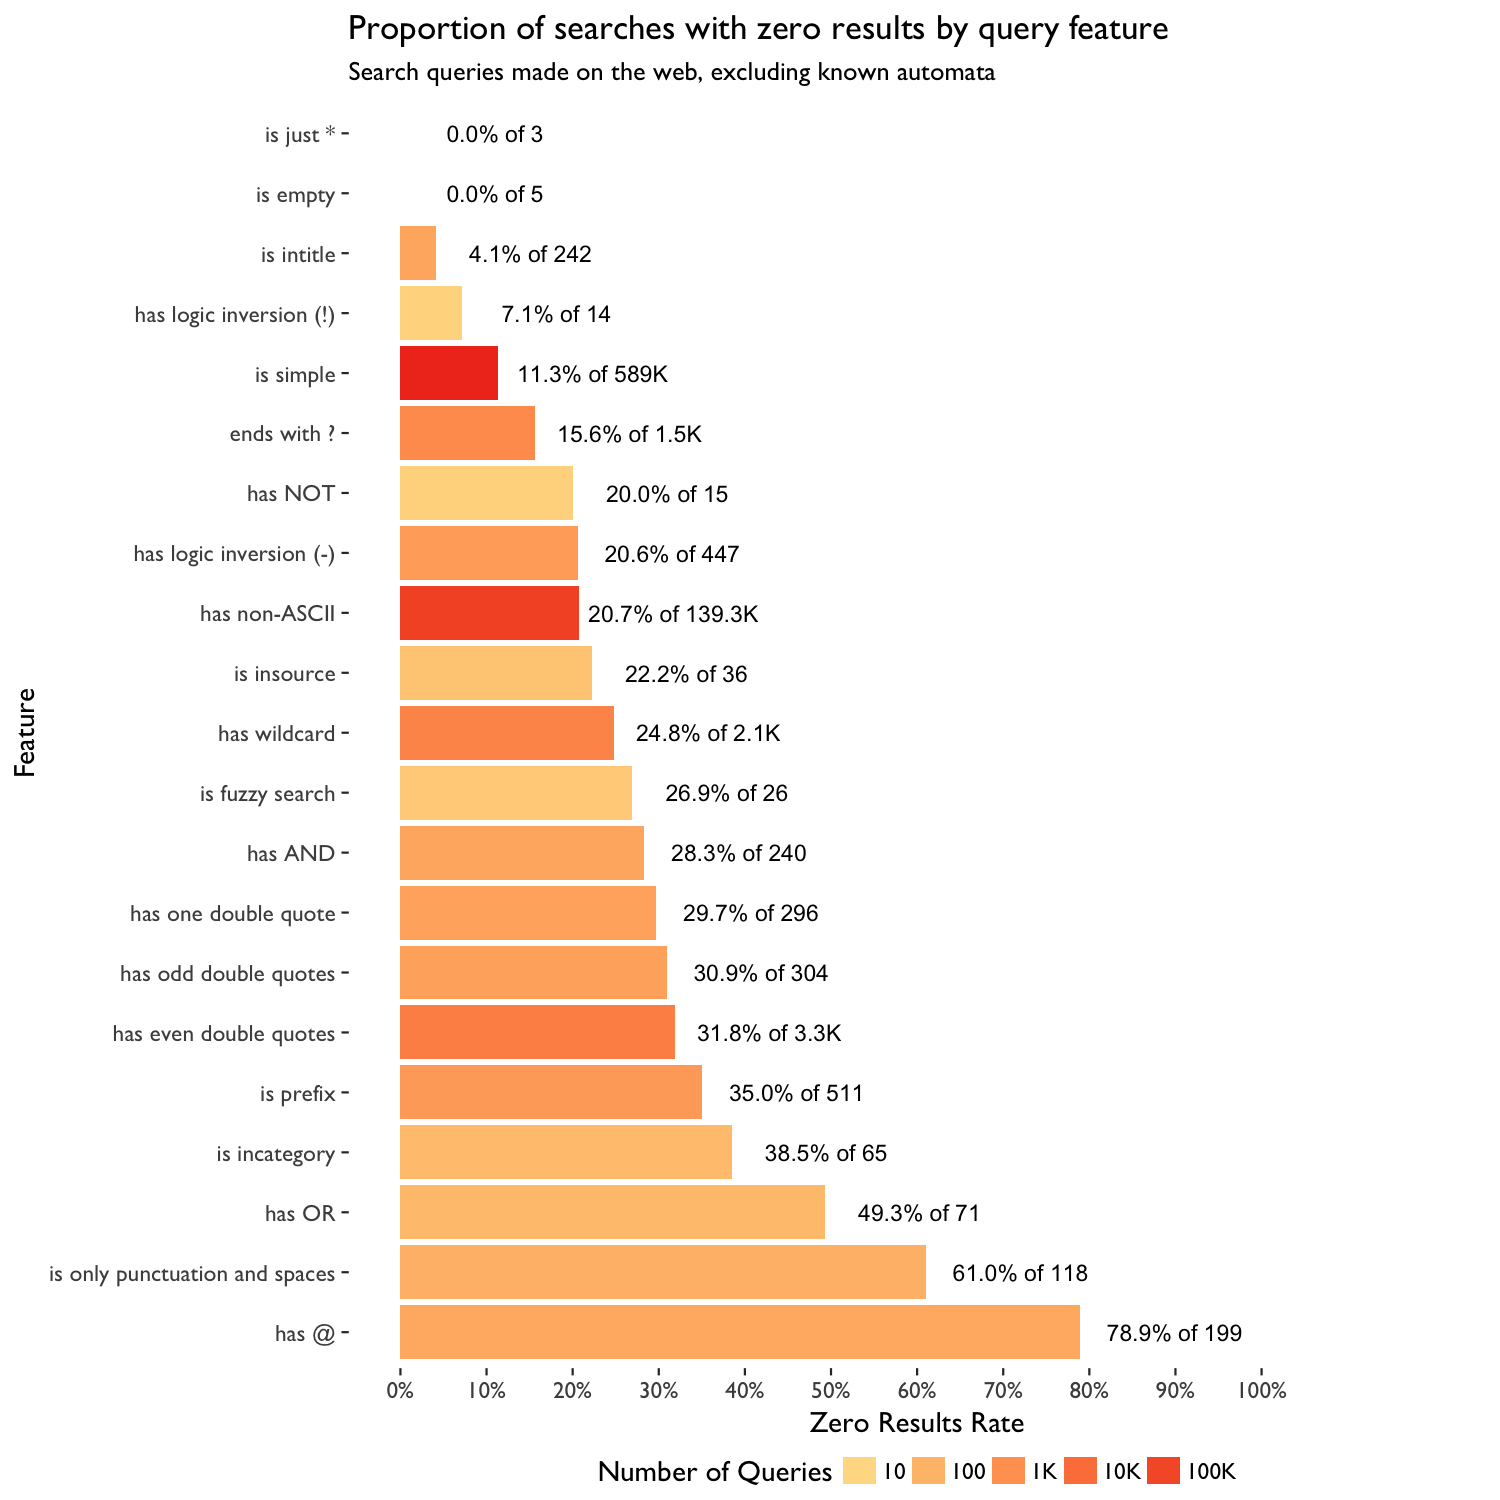
\includegraphics{figures/zrr_by_feature.png}
\caption{Zero results rate by extracted features.}
\end{figure}

\begin{figure}[htbp]
\centering
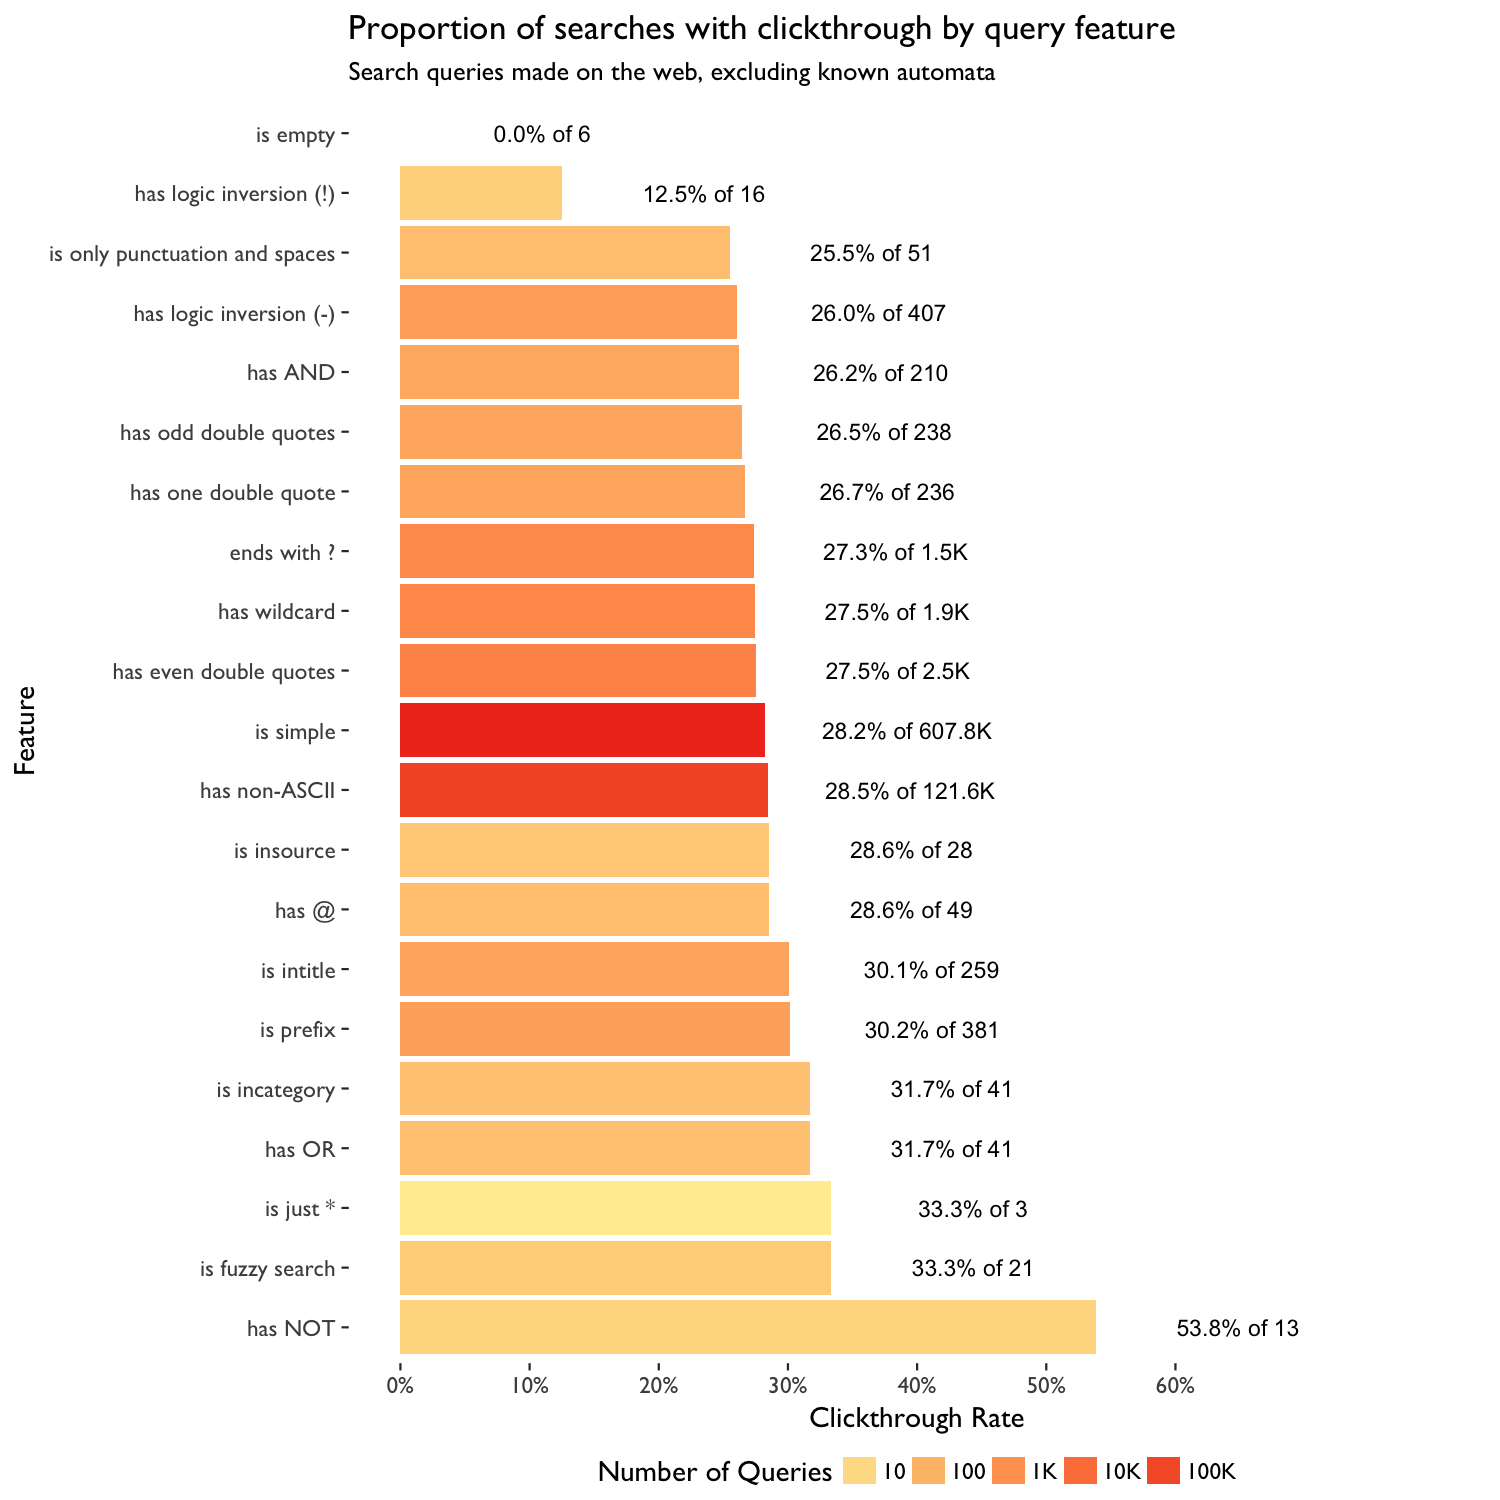
\includegraphics{figures/ctr_by_feature.png}
\caption{Clickthrough rate by extracted features.}
\end{figure}

\newpage

\begin{landscape}

\begin{figure}
\centering
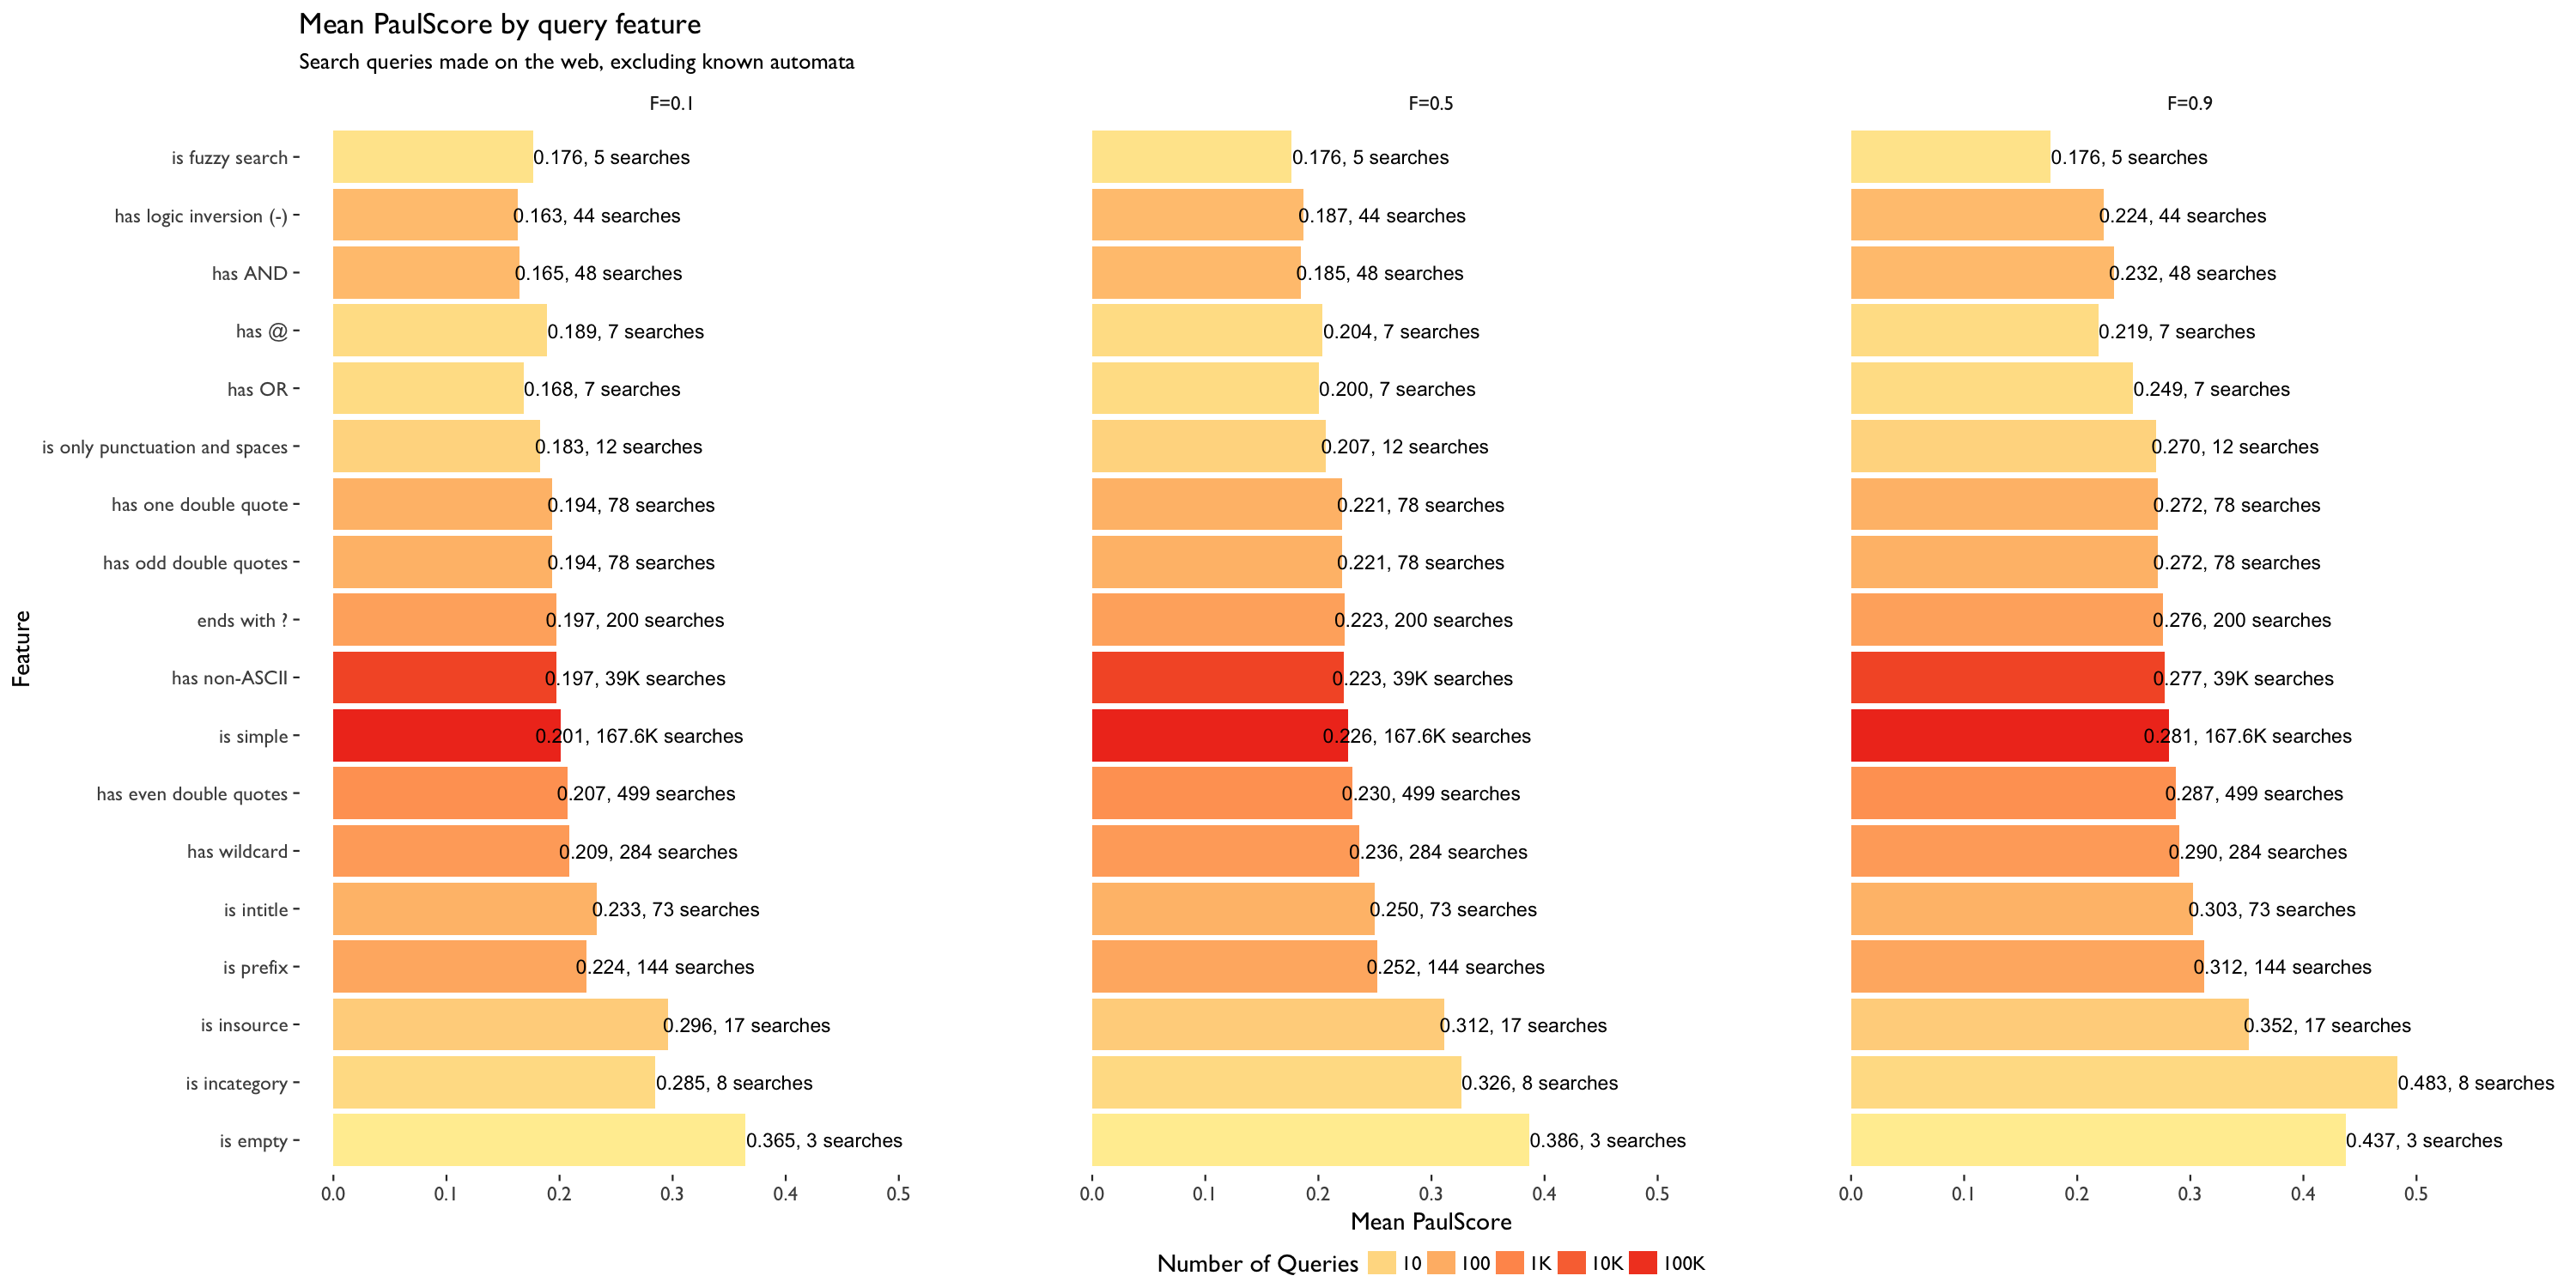
\includegraphics{figures/paulscore_by_feature.png}
\caption{Mean PaulScore by extracted features. Scoring factors are 0.1, 0.5 and 0.9 respectively.}
\label{fig:paulscore_by_feature}
\end{figure}

\end{landscape}

\newpage

\subsubsection{Zero Result Rate}\label{zero-result-rate}

\textbf{Random Forest}: Overall accuracy of test set is 0.7056147, AUC
is 0.7172. The confusion matrix is:

\begin{longtable}[]{@{}lrrr@{}}
\toprule
& some results & zero results & class error\tabularnewline
\midrule
\endhead
some results & 91057 & 36474 & 0.2860011\tabularnewline
zero results & 6750 & 12547 & 0.3497953\tabularnewline
\bottomrule
\end{longtable}

The following variable importance plot (Fig. 4) shows that ``has even
double quotes'' and ``is only punctuation and spaces'' are more
important than others when predicting zero result.

\textbf{Logistic Regression}: The two tuned parameter of elastic net
penalty are very closed to 0, which means logistic regression without
penalty works best here. Overall accuracy of test set is 0.6946972, AUC
is 0.6726. The confusion matrix is:

\begin{longtable}[]{@{}lrrr@{}}
\toprule
& some results & zero results & class error\tabularnewline
\midrule
\endhead
some results & 91441 & 36090 & 0.28299\tabularnewline
zero results & 8737 & 10560 & 0.45276\tabularnewline
\bottomrule
\end{longtable}

Fig. 5 compares the features using the measures from both models to
reveal which features the two models agree on. As before, we should pay
more attention to MDA specific to queries with zero results. We can see
that ``has even double quotes'' and ``is only punctuation and spaces''
are relatively more important and make zero result more likely.

\newpage

\begin{landscape}

\begin{figure}[h!]
\centering
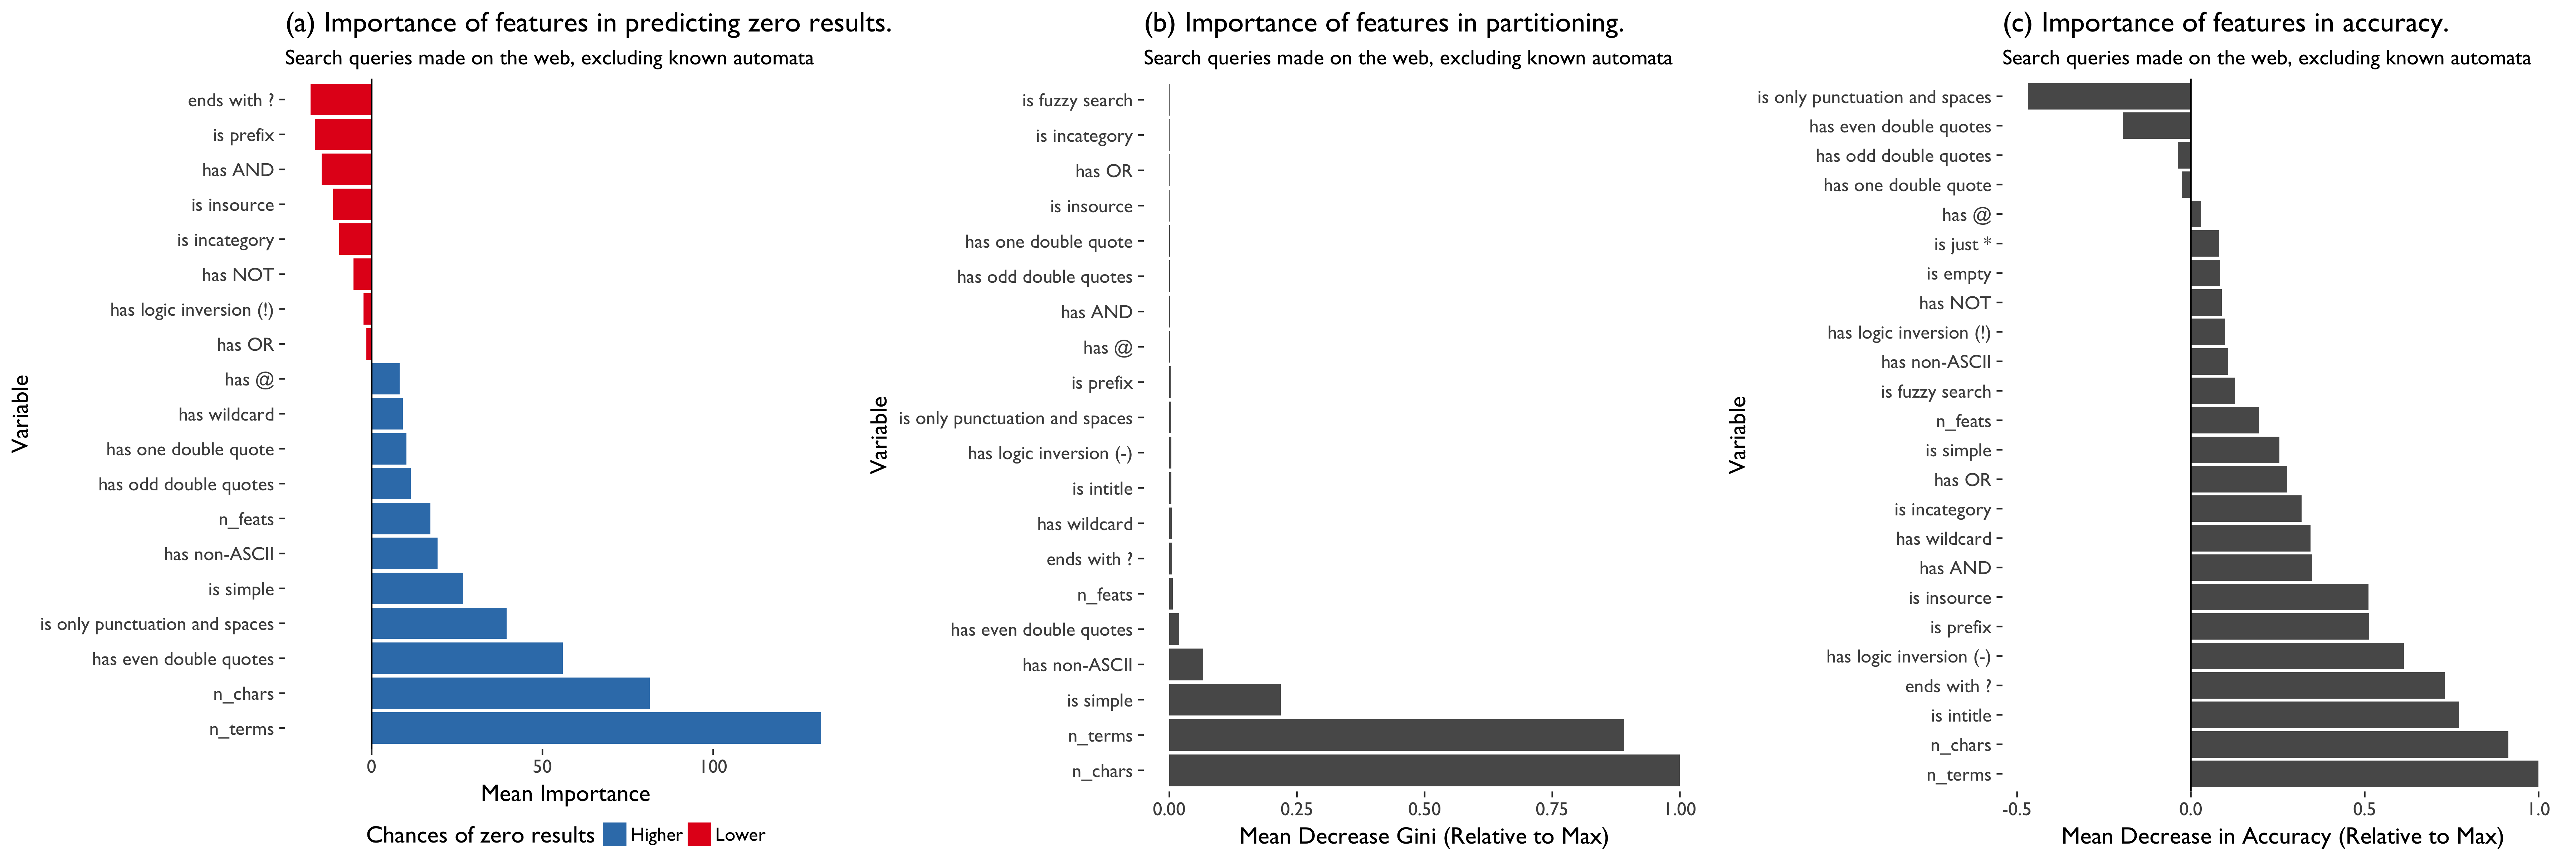
\includegraphics{figures/var_imp_zrr.png}
\caption{\textbf{(a)} Variable importance according to mean decrease in accuracy (increase in prediction error after permuting values of the predictor) specific to zero results queries. \textbf{(b)} Variable importance according to mean decrease in impurity, using Gini index. \textbf{(c)} Variable importance according to mean decrease in accuracy over both classes of queries (zero results and some results).}
\label{fig:var_imp_zrr}
\end{figure}

\end{landscape}

\newpage

\begin{landscape}

\begin{figure}[h!]
\centering
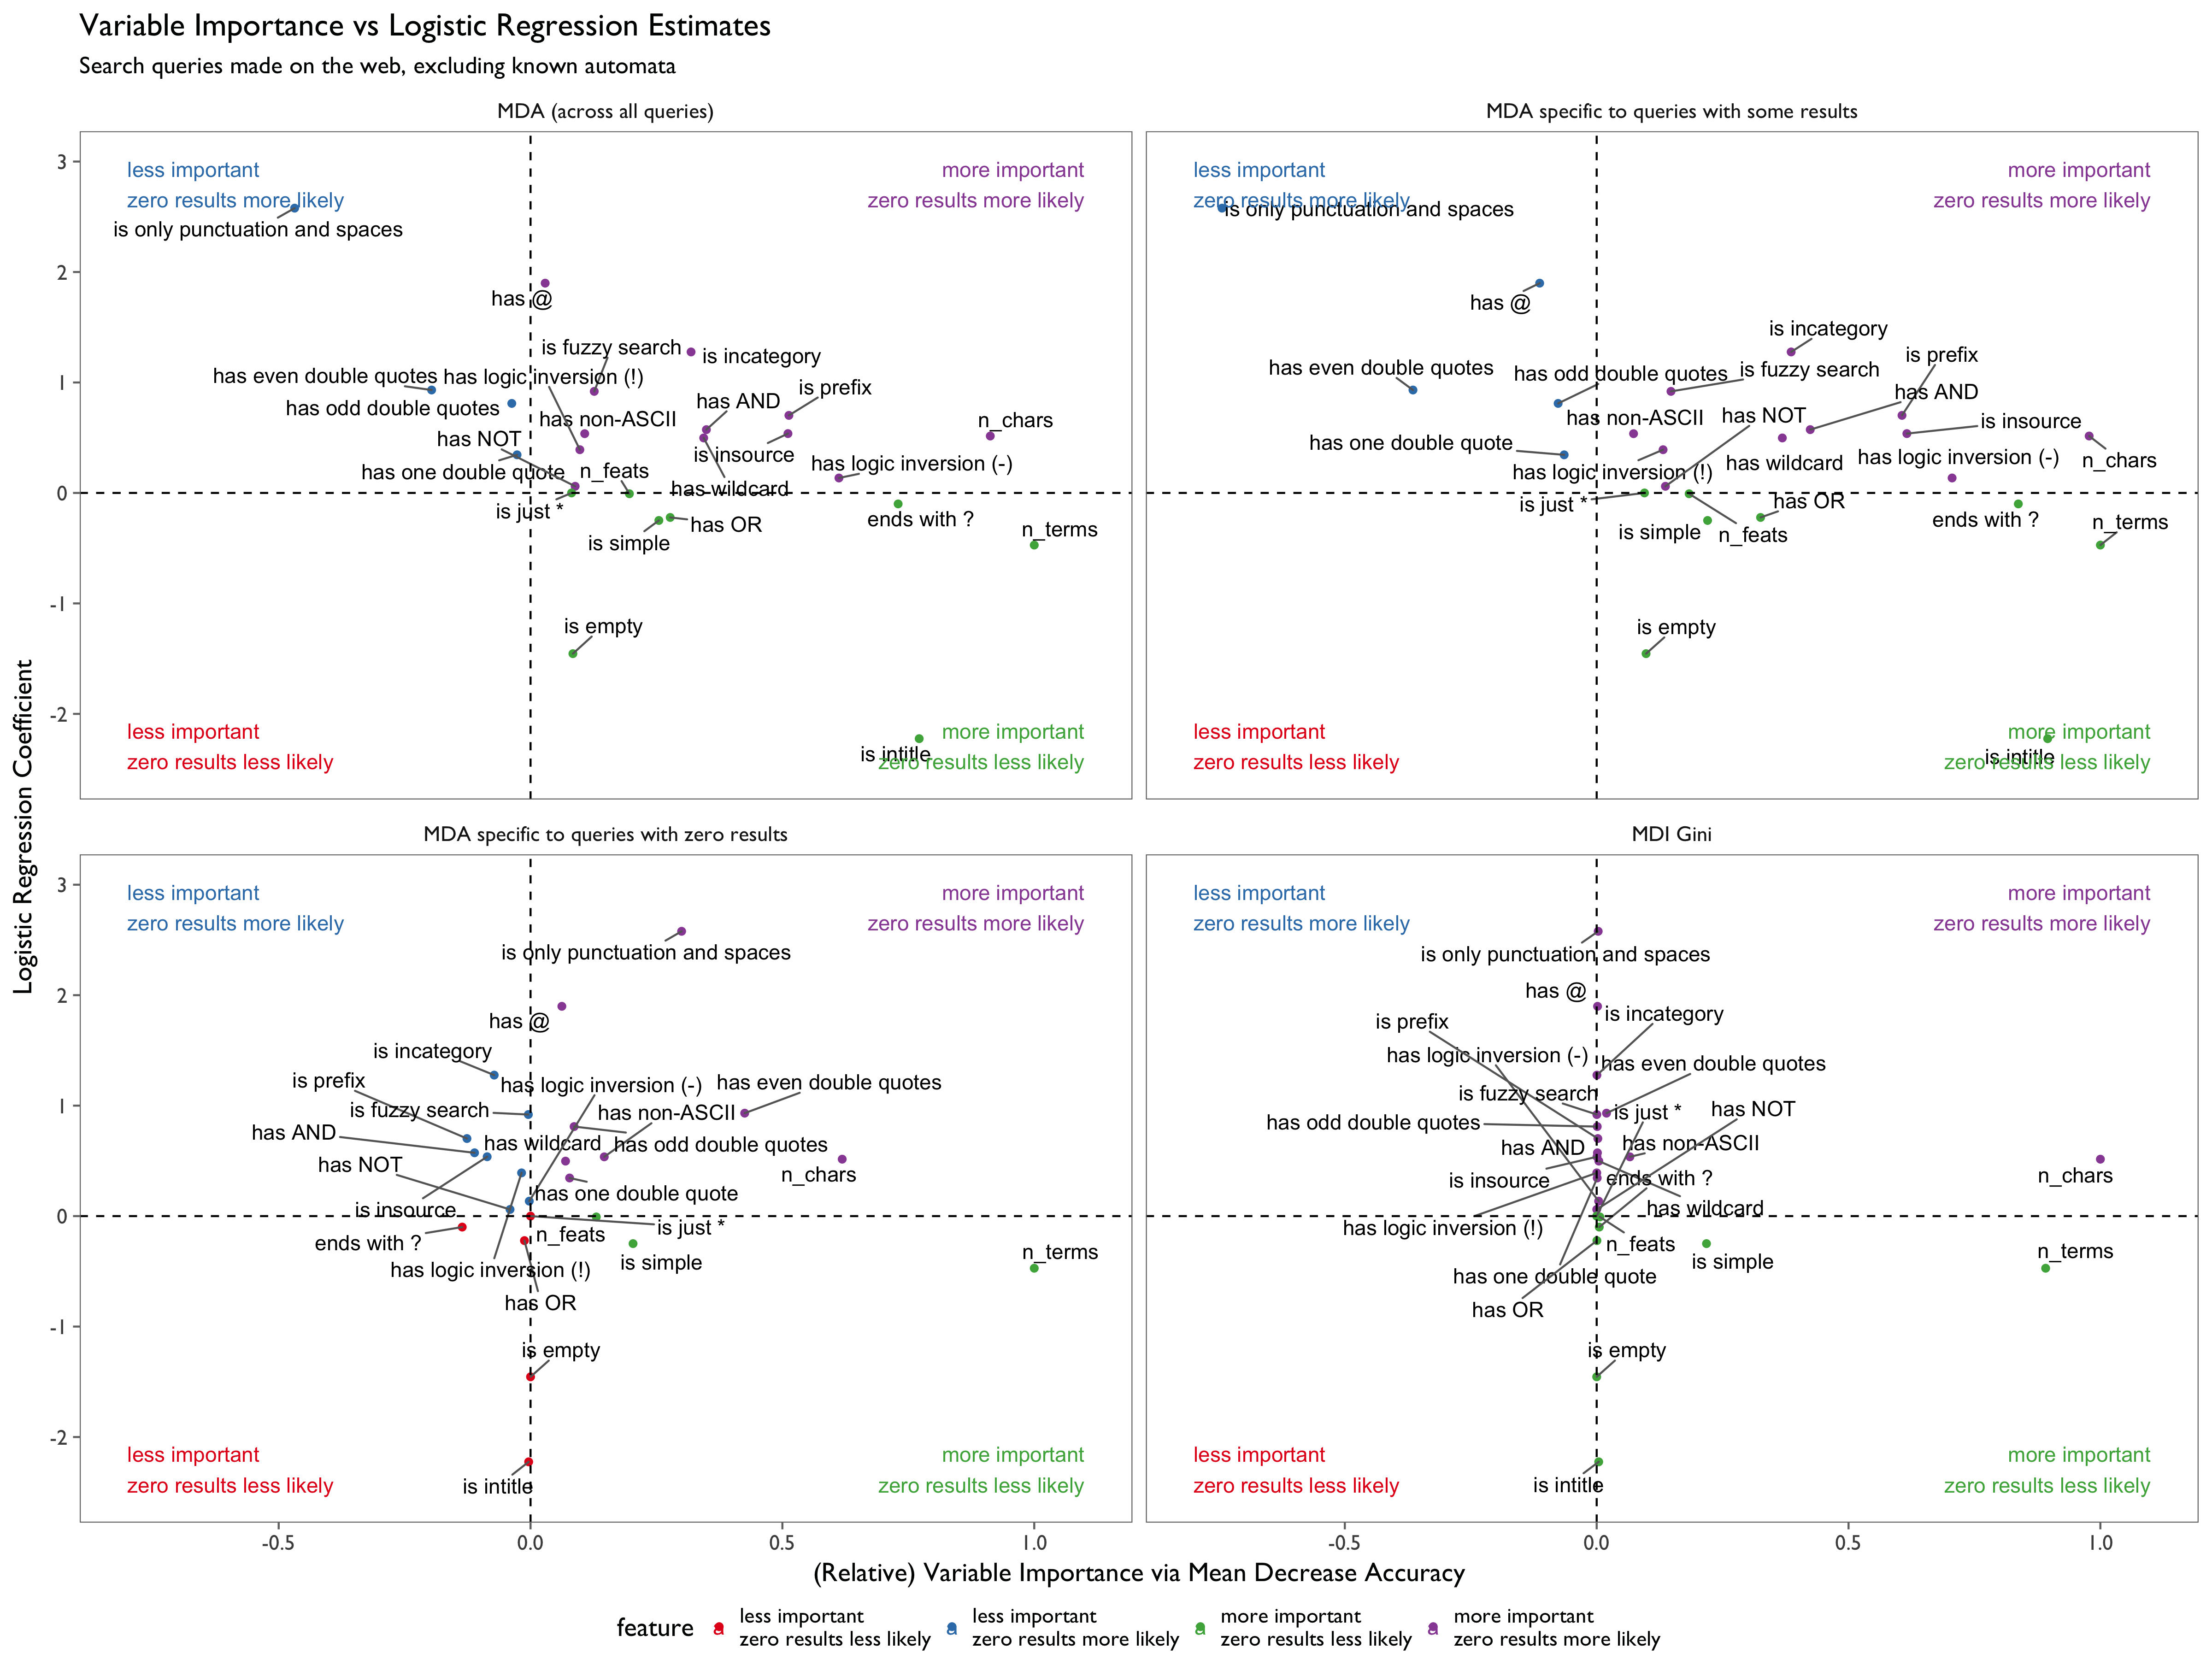
\includegraphics{figures/mda_logitcoef_zrr.png}
\caption{A scatter map of features with respect to variable importance (via relative mean decrease metrics) and logistic regression coefficient estimates. Each of the 4 plots is divided into quadrants according to how important or unimportant the feature is in random forest classification and whether a query having the feature is more or less likely to yield zero results.}
\label{fig:mda_logitcoef_zrr}
\end{figure}

\end{landscape}

\subsubsection{Clickthrough Rate}\label{clickthrough-rate}

\textbf{Random Forest: } Overall accuracy of test set is 0.4399294, AUC
is 0.5004, which means the model is not very useful. The confusion
matrix is:

\begin{longtable}[]{@{}lrrr@{}}
\toprule
& zero click & clickthrough & class error\tabularnewline
\midrule
\endhead
zero click & 23986 & 61909 & 0.7207521\tabularnewline
clickthrough & 9444 & 32061 & 0.2275389\tabularnewline
\bottomrule
\end{longtable}

\textbf{Logistic Regression: } Overall accuracy of test set is
0.4801099, AUC is 0.5314. The confusion matrix is:

\begin{longtable}[]{@{}lrrr@{}}
\toprule
& zero click & clickthrough & class error\tabularnewline
\midrule
\endhead
zero click & 35255 & 50640 & 0.589557\tabularnewline
clickthrough & 15594 & 25911 & 0.375714\tabularnewline
\bottomrule
\end{longtable}

Because AUC is too close to 0.5, and the class error for zero click is
too large, we do not think query features have large enough predictive
power on clickthrough rate, and thus we are not reporting variable
importance here (see appendix below).

\subsubsection{PaulScore}\label{paulscore}

\textbf{Linear Regression: } We fit linear regression models (lambdas of
elastic net penalty are very close to 0) for PaulScore when scoring
factor equals 0,1, 0.5 and 0.9. The explained deviance by models are
very small, less than 0.3\%, and R squared ranges from 0.005 to 0.009.
Therefore, we do not think query features have enough predictive power
on PaulScore, and thus we are not reporting variable importance here.

\textbf{Random Forest: } Random forest regression did a little bit
better than linear regression, but the performance measures are still
too small: The R squared of test set are 0.014, 0.011 and 0.0013, the
mean squared errors are 0.986, 0.989 and 0.999, for PaulScore when
scoring factor equals 0,1, 0.5 and 0.9 respectively. Therefore, we do
not think query features have enough predictive power on PaulScore, and
thus we are not reporting variable importance here.

\begin{landscape}

\subsection{Appendix}

\begin{figure}[h!]
\centering
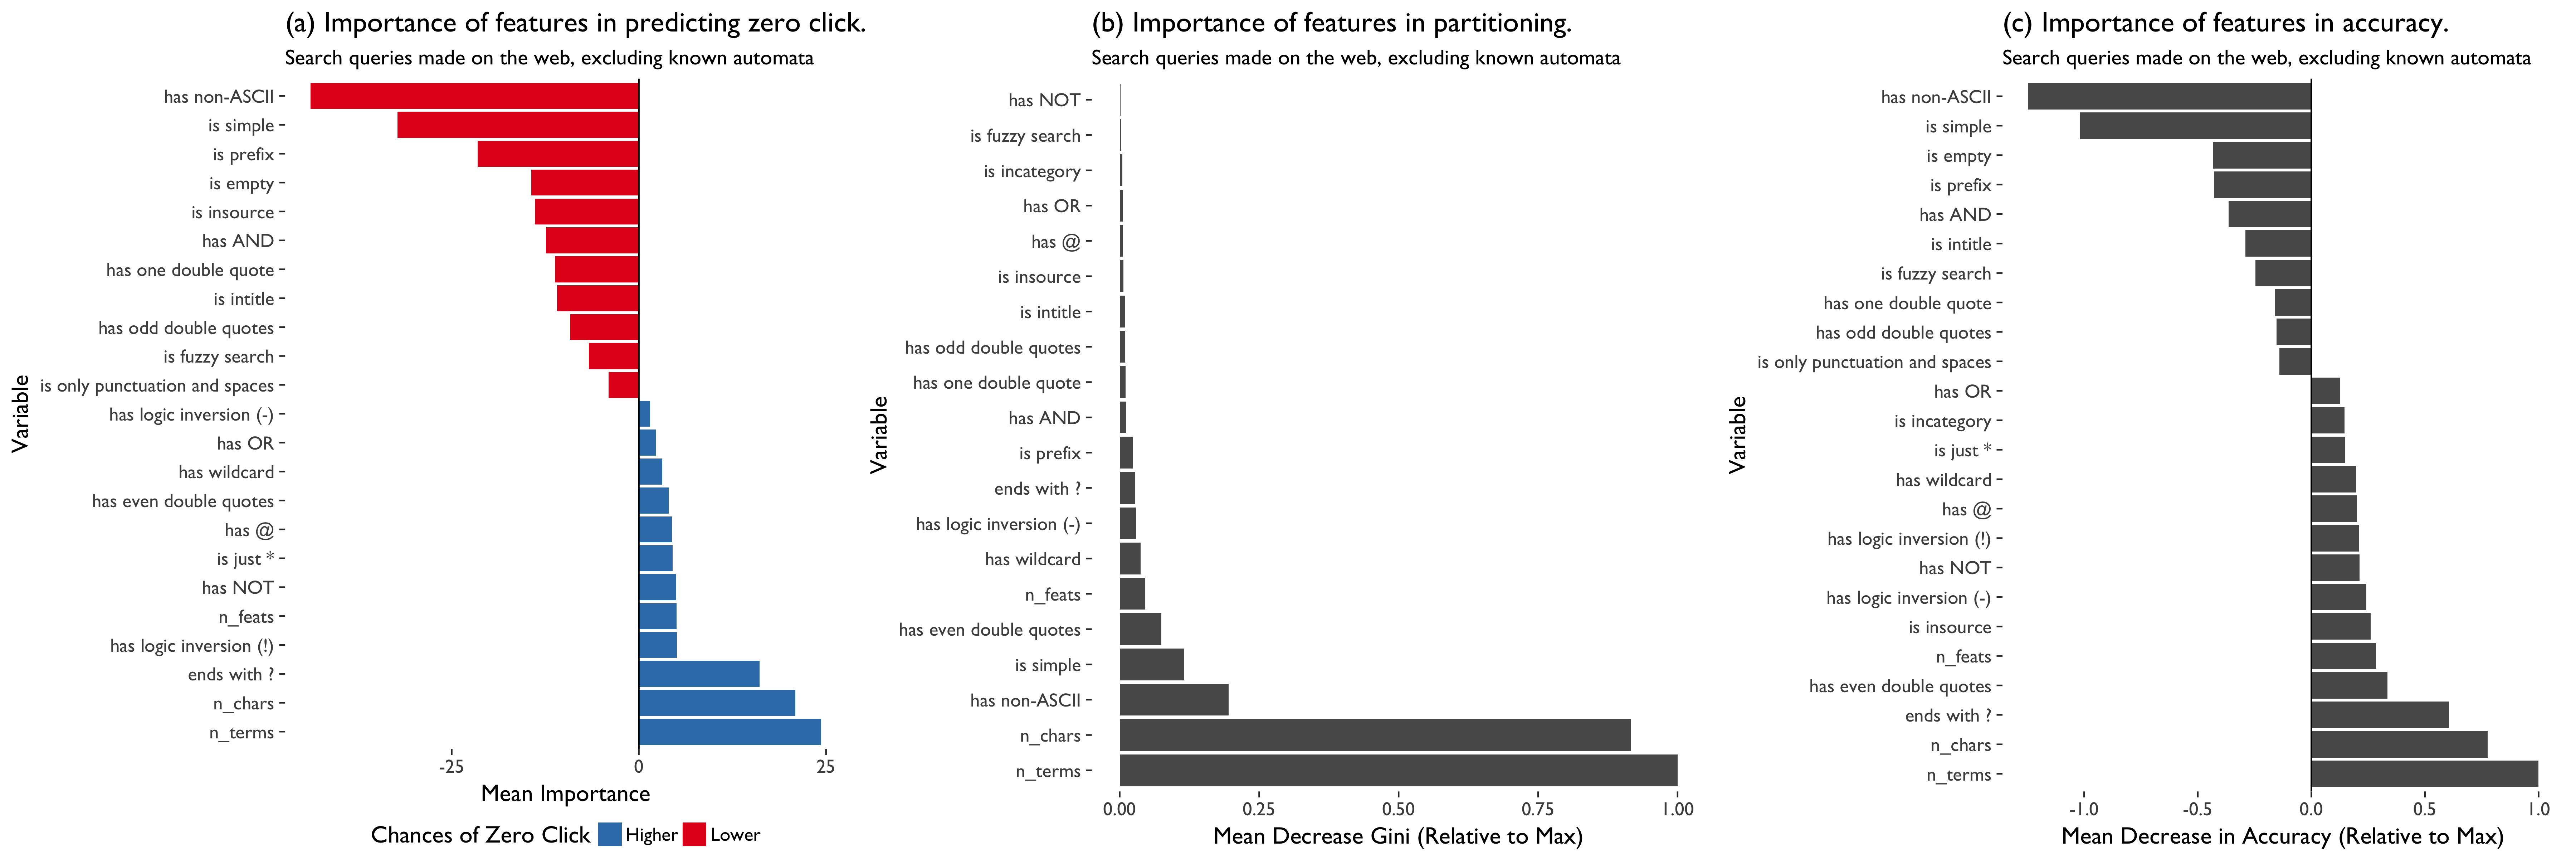
\includegraphics{figures/var_imp_ctr.png}
\caption{\textbf{(a)} Variable importance according to mean decrease in accuracy (increase in prediction error after permuting values of the predictor) specific to zero click queries. \textbf{(b)} Variable importance according to mean decrease in impurity, using Gini index. \textbf{(c)} Variable importance according to mean decrease in accuracy over both classes of queries (zero click and clickthrough).}
\label{fig:mda_coef}
\end{figure}

\begin{figure}[h!]
\centering
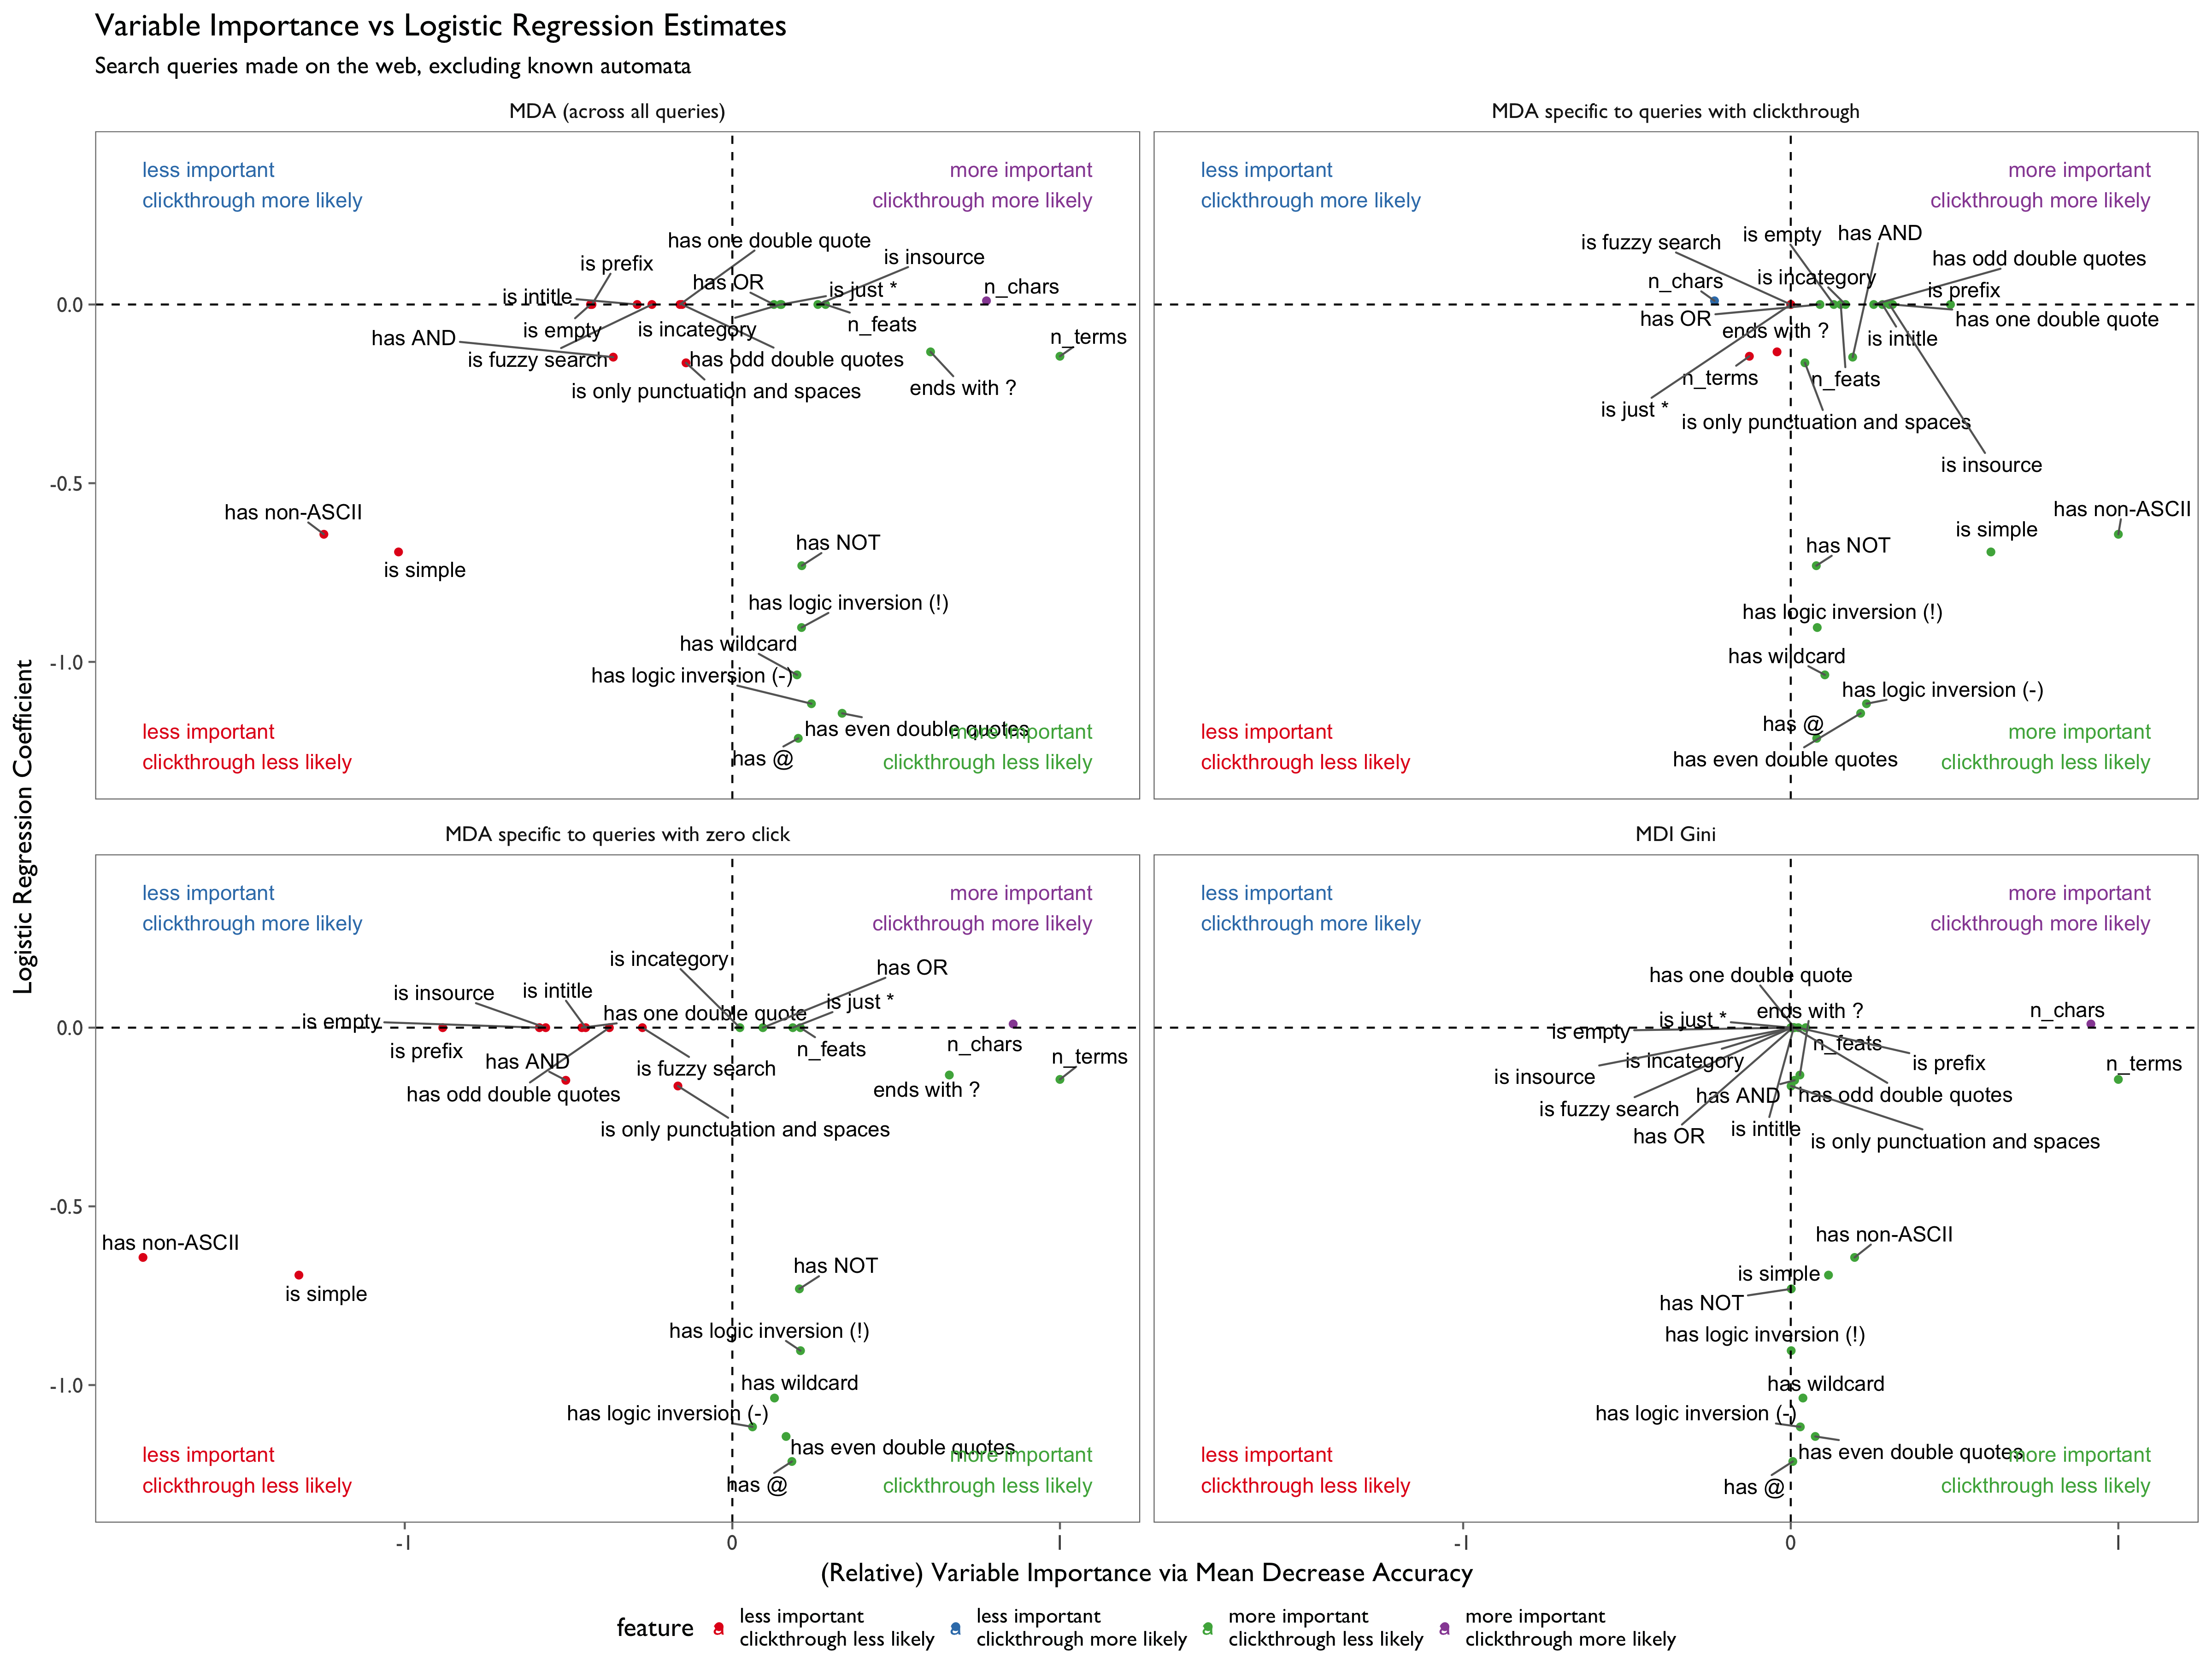
\includegraphics{figures/mda_logitcoef_ctr.png}
\caption{A scatter map of features with respect to variable importance (via relative mean decrease metrics) and logistic regression coefficient estimates. Each of the 4 plots is divided into quadrants according to how important or unimportant the feature is in random forest classification and whether a query having the feature is more or less likely to yield at least one click.}
\label{fig:mda_coef}
\end{figure}

\end{landscape}


\end{document}
